\documentclass[journal,12pt,onecolumn,draftcls]{IEEEtran}
\usepackage{amsmath,amssymb,amsfonts}
\usepackage{algorithmic}
\usepackage{graphicx}
\usepackage{xcolor}
\newcommand{\editornote}[1]{\par\textit{\textcolor{blue}{\textbf{Editor's Note:} #1}}\par}
\usepackage{float}
\usepackage{setspace}
\usepackage{hyperref}
\usepackage{makecell}

\hypersetup{
      colorlinks=true,
      linkcolor=blue,
      citecolor=black,      
      urlcolor=blue
}

\doublespacing

\begin{document}
\title{One-Class Autoencoder for Anomaly Detection of Malaria Infected Cells}
\author{\IEEEauthorblockN{Author Name}}
\maketitle
\begin{abstract}
  Malaria remains a major public health challenge, especially in developing regions where diagnostic resources are limited. Traditional detection methods often suffer from low sensitivity and require expert interpretation. In this study, we propose a one-class autoencoder trained exclusively on normal red blood cell images to learn their latent structure and identify anomalous deviations associated with malaria infection. Using structural similarity (SSIM) as the primary evaluation metric, our method demonstrates strong classification performance on two microscopy datasets. These results highlight the potential of unsupervised learning in enhancing automated malaria diagnosis, particularly in resource-constrained settings.
\end{abstract}

\editornote{
(0a) Hyphenated “one class autoencoder” as “one-class autoencoder” to conform to compound modifier conventions in IEEE style;
(0b) Rephrased “malaria detection methods” and “solution for malaria detection” to avoid redundancy and improve concision;
(0c) Recast vague phrases such as “learn underlying patterns and identify deviations” into more precise technical language describing latent structure and anomaly detection;
(0d) Added mention of the SSIM evaluation metric and dual-dataset validation to enhance specificity and credibility;
(0e) Replaced general claims like “high accuracy” with more contextualized performance framing (“strong classification performance”) to preserve objective tone.
}

\begin{IEEEkeywords}
anomaly detection, malaria detection, deep learning, one class autoencoders
\end{IEEEkeywords}

\section{Problem Statement}
Malaria is a life-threatening disease caused by parasites transmitted to people through the bites of infected mosquitoes. The \textit{World Malaria Report 2022} highlights that there were an estimated 247 million malaria cases in 2021 in 84 endemic countries \cite{who2022}, with most of the increase coming from countries in the African Region of the World Health Organization (WHO). Malaria case incidence declined from 82 in 2000 to 57 in 2019, before increasing to 59 in 2020, with no change in case incidence between 2020 and 2021. The increase in 2020 was associated with disruptions to services during the COVID-19 pandemic, which led to an estimated additional 13.4 million cases between 2019 and 2021. Twenty-nine countries accounted for 96\% of global malaria cases, with Nigeria, the Democratic Republic of the Congo, Uganda, and Mozambique accounting for nearly half. The African Region, with an estimated 234 million cases in 2021, accounted for about 95\% of global cases \cite{who2022}.

\editornote{(1a) Introduced “World Health Organization (WHO)” on first mention to define the acronym; 
(1b) Rephrased “WHO African Region” to “the African Region of the World Health Organization (WHO)” for structural clarity; 
(1c) Replaced comma splice with a period before “Twenty-nine countries...” to separate independent clauses; 
(1d) Replaced “29” with “Twenty-nine” to conform to IEEE guidance on numerals at the start of sentences; 
(1e) Reworded “accounting for almost half” to “accounting for nearly half” for a more measured, technical phrasing; 
(1f) Replaced “reduced” with “declined” for correct intransitive verb usage in epidemiological context; 
(1g) Removed repeated “WHO” in final sentence for conciseness and to avoid acronym redundancy.}

Malaria continues to pose a significant public health challenge, particularly in developing countries, where access to diagnostic tools and treatment is often limited. Current diagnostic methods for malaria detection, such as microscopy and rapid diagnostic tests \cite{wilson2012}, have several limitations, including variability in diagnostic sensitivity and specificity, high costs, and dependence on skilled personnel. As such, the development of more accurate and efficient methods for malaria detection—particularly in resource-limited settings—is critical.

\editornote{(2a) Changed “can be limited” to “is often limited” for more direct phrasing and improved flow; 
(2b) Added comma after “high costs” to maintain parallel structure in the list; 
(2c) Replaced “cost” with “costs” to match the plural form used for “limitations”; 
(2d) Replaced commas around “particularly in resource-limited settings” with em dashes to visually set off the clause and reduce comma stacking.}

To address these challenges, we turn to anomaly detection, also known as outlier detection—a technique used to identify rare or unexpected observations or patterns in a dataset \cite{chandola2009}, \cite{ruff2021}, \cite{edgeworth1887}. Anomaly detection offers a promising avenue for improving malaria diagnostics. It is widely applied in fields such as finance, cybersecurity, and medical diagnosis, where identifying irregularities is critical for detecting fraud, uncovering network intrusions, or diagnosing diseases. This concept has proven useful in identifying the presence of the malaria parasite in cell images.

\editornote{(3a) Recast “It is a technique that is used...” as “a technique used...” for conciseness and to eliminate redundancy; 
(3b) Combined first two sentences using an em dash to reduce fragmentation and improve flow; 
(3c) Removed repetition of “It is” at the beginning of multiple sentences to vary structure and tone; 
(3d) Replaced “detecting anomalies is crucial for detecting...” with “identifying irregularities is critical for...” to avoid repetition and elevate register; 
(3e) Clarified “presence of malaria virus” as “malaria parasite,” which is biologically more accurate. Specifically, malaria is caused by protozoan parasites of the genus Plasmodium.}

In this research endeavor, we propose a one-class methodology for the classification of red blood cells depicted in microscopic images. This approach leverages normal cell images to address a common challenge in medical imaging: the insufficient number of abnormal or infected instances.

\editornote{(4a) Replaced “propose the utilization of” with “propose” to reduce verbosity; 
(4b) Hyphenated “one class” as “one-class” to follow compound modifier convention; 
(4c) Reworded sentence two for clarity, shifting from “solve a commonly encountered challenge...” to “address a common challenge...” for conciseness; 
(4d) Replaced “which is” with a colon to streamline the clause and improve flow.}

One-class anomaly detection is a machine learning technique that is particularly useful for identifying anomalous instances within a single class of data. By training a model on a large and diverse dataset of normal instances, the proposed method can extract deep features that distinguish normal from anomalous cases. These features can be learned using deep learning models such as autoencoders and convolutional neural networks (CNNs), which capture hierarchical representations of image data, including both global and local patterns \cite{torres2021}.

\editornote{(5a) Hyphenated “One class” to “One-class” as a compound modifier; 
(5b) Corrected “instance” to plural “instances” to match the plural subject; 
(5c) Replaced “should be able to” with “can” for conciseness and consistency with previous edits; 
(5d) Removed second occurrence of “deep features” to avoid repetition and tighten phrasing; 
(5e) Simplified final clause by replacing “in instances where images are used” with “of image data,” and clarified it with “global and local patterns” for readability and flow.}

Deep learning, which falls under the umbrella of machine learning, involves creating computer models capable of learning patterns and making predictions. What sets deep learning apart is its ability to automatically recognize important features in data without requiring experts to manually identify the most relevant information. These capabilities make deep learning especially valuable in fields like medical imaging. In areas where it is difficult to determine which parts of an image are diagnostically important—such as disease classification and tumor detection—deep learning models excel at interpreting complex data, making them powerful tools in healthcare and beyond \cite{torres2021}.

\editornote{(6a) Added commas around the clause “which falls under the umbrella of machine learning” to set it off properly; 
(6b) Replaced “teach artificial intelligence systems” with “learning patterns and making predictions” for technical precision; 
(6c) Changed “tough to figure out” to “difficult to determine” to maintain formal tone; 
(6d) Reworded “making sense of complex data, making them...” to avoid repetition and improve rhythm; 
(6e) Added “diagnostically” to clarify the medical context of visual interpretation.}

In summary, the major solutions that this proposal seeks to solve are:
\begin{itemize}
  \item \textbf{Addressing Data Scarcity:} This approach tackles the persistent challenge of limited abnormal samples in medical imaging by leveraging normal cell images to train a robust detection model.
  \item \textbf{Reducing False Positives:} The method leads to fewer false alarms—an essential benefit in domains such as medical diagnostics and fraud detection, where false positives can have serious consequences.
\end{itemize}

\editornote{(7a) Edited bullet labels to follow parallel grammatical structure using gerunds (“Addressing,” “Reducing”); 
(7b) Reworded item descriptions to reduce redundancy and increase technical clarity; 
(7c) Replaced vague phrasing (“It tackles the significant challenge...”) with more precise language; 
(7d) Emphasized domain relevance (“medical diagnostics and fraud detection”) to align with professional tone and context.}

Through this research, we demonstrate that our one-class autoencoder achieves above-average accuracy in detecting infected cells in microscopic images. This result highlights the model’s potential as a reliable tool for improving malaria diagnosis and strengthening healthcare delivery, especially in resource-limited settings.

\editornote{(8a) Recast “we show that our approach demonstrates” as “we demonstrate that our approach achieves” for directness and assertiveness; 
(8b) Substituted “makes our model a promising and reliable tool” with “highlights the model’s potential as a reliable tool” for smoother flow and more objective tone; 
(8c) Replaced “enhancing healthcare outcomes” with “strengthening healthcare delivery” for specificity and alignment with medical/public health terminology.}

\section{Literature Review}
Bobde et al. \cite{bobde2022} proposed an autoencoder model for malaria cell classification. They trained the model on image data and froze the encoder to extract features. The encoder was then integrated with fully connected convolutional neural network (CNN) layers and used a softmax activation function for binary classification. After fine-tuning, the model was deployed in a user-friendly web application, demonstrating its practical applicability—even for users with minimal technical training.

\editornote{(9a) Removed “algorithm” after “autoencoder” to avoid redundancy; 
(9b) Rephrased “to address the malaria cell classification problem” as “for malaria cell classification” to improve conciseness; 
(9c) Reworded “training it with data” as “trained the model on image data” for specificity and clarity; 
(9d) Clarified and formalized the final sentence by changing “showcasing its real-life applicability...” to “demonstrating its practical applicability...” and added “technical” before “training” for precision.}

Autoencoders are unsupervised learning models that compress input data into a lower-dimensional latent representation and reconstruct the original input from it. Composed of encoder, bottleneck, and decoder components, they uncover coherent structures in the data and serve as domain-specific, lossy dimensionality reduction tools. In this study, the encoder was used as a feature extractor to identify relevant patterns in blood sample images for classification. The study also incorporated convolutional neural networks (CNNs), which are biologically inspired models capable of assigning importance to features and capturing spatial and temporal dependencies through learned filters. Their hierarchical structure makes them well-suited for image analysis tasks.

\editornote{(10a) Replaced “an unsupervised learning algorithm” with “unsupervised learning models” to match plural subject; 
(10b) Reworded “lower-dimensional code” as “latent representation” for technical precision; 
(10c) Rephrased “comprising encoder, code, and decoder” as “composed of encoder, bottleneck, and decoder components” for clarity and terminology accuracy; 
(10d) Removed repeated mention of “unsupervised” to streamline explanation; 
(10e) Clarified and formalized final CNN sentence by specifying “hierarchical structure” as justification for effectiveness in image tasks.}

To evaluate model performance, metrics were recorded across the training, validation, and testing phases, including accuracy, loss, precision, recall, and F1 score. An EarlyStopping callback was used to minimize overfitting and conserve computational resources. The model achieved a training accuracy of 96.06\%, a validation accuracy of 96.52\%, and a testing accuracy of 95.31\%. Training ran for 84 epochs, halting automatically after approximately four hours due to the EarlyStopping criterion. These results indicate a high degree of robustness and classification effectiveness in the context of malaria cell detection.

\editornote{(11a) Condensed opening clause to “To evaluate model performance...” for clarity and brevity; 
(11b) Lowercased “F1 Score” to “F1 score” to match standard formatting; 
(11c) Merged two mentions of “EarlyStopping callback” for improved cohesion; 
(11d) Replaced “The results were impressive” with a more objective summary; 
(11e) Repositioned “approximately four hours” earlier in the sentence for logical flow; 
(11f) Clarified final sentence by specifying “classification effectiveness” and reinforcing the medical domain.}

Musa et al. \cite{musa2022} proposed a convolutional neural network (CNN) architecture for classifying malaria cells using blood image data. The sixteen-layer model demonstrated strong performance, achieving an average accuracy of 97.37\% during ten-fold cross-validation. It also achieved a classification accuracy of 94\% on individual test images.

\editornote{(12a) Removed “thereby indicating whether or not an individual has malaria” as redundant, given the classification context; 
(12b) Rephrased “CNN model” to “CNN architecture” to avoid redundancy and better reflect research conventions; 
(12c) Combined “remarkable efficacy” and “impressive accuracy” into a single, objective statement to remove subjective language; 
(12d) Clarified “boasting a high classification accuracy” as “achieved a classification accuracy” for formal tone and reduced repetition.}

The experimental phase of the convolutional neural network (CNN) approach involved testing various activation functions and training durations to optimize accuracy. The optimal configuration used ReLU as the first activation function, sigmoid as the second, Adam as the optimizer, and 25 training epochs, resulting in a classification accuracy of 95.6\%.

\editornote{(13a) Rephrased “experimental phases of the Convolutional Neural Network (CNN) approach” to “experimental phase of the CNN approach” for conciseness; 
(13b) Replaced “to enhance accuracy” with “to optimize accuracy” to align with technical terminology; 
(13c) Condensed “most effective configuration from the experiments” to “optimal configuration”; 
(13d) Removed “impressive” to eliminate subjective evaluation and maintain objective tone; 
(13e) Specified “25 epochs” as “25 training epochs” for clarity.}

Reddy et al. \cite{reddy2021} developed a system that combined Inception v3, a transfer learning model, with a support vector machine (SVM) classifier for malaria detection. Inception v3 was used to extract features, which were then classified by the SVM. As part of Google’s deep learning architecture family, Inception v3 provided a powerful convolutional backbone for visual feature extraction.

\editornote{(14a) Lowercased “Transfer Learning model” to “transfer learning model” to match technical conventions; 
(14b) Simplified phrasing of feature extraction and classification by collapsing two redundant clauses; 
(14c) Replaced subjective “pivotal” and “potent” with less subjective phrasing; 
(14d) Substituted “component of Google’s Deep Learning Architecture series” with “part of Google’s deep learning architecture family” as I believe the architecture's formal title is the Inception architecture series, with version numbering starting after GoogleNet as the original version. I opted for a less specific titling to avoid confusion, but confer with the author on this point.}

The model was frozen up to its bottleneck layer, located just below the fully connected layer. During training, it achieved an accuracy of 93\%, and in the final testing stage, it reached 94.8\%, reflecting consistent performance across phases.

\editornote{(15a) Retained and clarified phrasing “frozen up to its bottleneck layer” for accuracy and flow; 
(15b) Replaced subjective descriptors “impressive” and “remarkable” with neutral reporting of results; 
(15c) Consolidated performance reporting into a single sentence to reduce redundancy; 
(15d) Reworded “throughout the training phase” to “during training” for precision.}

\section{Dataset}
This study is based on a dataset derived from Giemsa-stained thin blood smear slides \cite{chakradeo2020}. The dataset includes samples collected at Chittagong Medical College Hospital in Bangladesh from 150 patients infected with *Plasmodium falciparum* and 50 healthy individuals.

\editornote{(16a) Rephrased “In this proposal, our research framework is rooted in...” to “This study is based on...” for conciseness and to match prior stylistic choices; 
(16b) Removed “compiled” and “obtained” as redundant phrasing; 
(16c) Replaced “painstakingly collected” with a neutral descriptor to maintain objective scientific tone; 
(16d) Expanded “P. falciparum” to “*Plasmodium falciparum*” on first use for clarity and biological specificity.}

The core dataset used in this study is the Malaria Detection dataset, available on IEEEDataPort under the title “Malaria Dataset (Thin Blood Smear, Updated).” Although valuable, the dataset contained a substantial number of mislabeled images. To address this, researchers conducted a manual review and relabeling process. The final dataset was reorganized into several groups, with a focus on two primary categories: uninfected and parasitized cells.

\editornote{(17a) Replaced “meticulously curated” with “used in this study” and clarified the dataset source and title for neutral tone and clarity; 
(17b) Reworded “considerable number of inaccurately labeled images” as “substantial number of mislabeled images” for conciseness and objectivity; 
(17c) Recast “a review and relabeling process was undertaken” into active voice as “researchers conducted a manual review and relabeling process” to improve clarity and engagement; 
(17d) Clarified “several groups with two pivotal categories” as “reorganized into several groups, with a focus on two primary categories” to improve precision.}

To supplement the primary dataset, a secondary dataset from Kaggle was incorporated into the study \cite{kaggle}. It comprises two classes of uninfected cells—red blood cells (RBCs) and leukocytes—and four classes of infected cells: gametocytes, rings, trophozoites, and schizonts. Some cells were annotated as “difficult” when they could not be clearly assigned to a single category. The dataset exhibited a strong class imbalance, with uninfected RBCs accounting for over 95\% of all cells.

\editornote{(18a) Reworded “as part of our broader dataset utilized for the deep learning model” to “To supplement the primary dataset” for conciseness and flow; 
(18b) Changed “we incorporated... into our research” to passive “was incorporated into the study” to maintain consistency with prior tone; 
(18c) Replaced “includes” with “comprises” and clarified cell classes using em dashes for uninfected and colon for infected for structural clarity; 
(18d) Recast “Annotators were allowed to mark” as “Some cells were annotated as ‘difficult’...” for neutrality and smoother flow; 
(18e) Rephrased final sentence to emphasize class imbalance and quantify RBC prevalence more directly.}

For training on the Kaggle dataset, we leveraged the provided bounding box coordinates to crop and categorize cells into two primary groups: uninfected and infected. This step enabled us to focus on regions of interest within the images and to streamline the training process.

\editornote{(19a) Capitalized “Kaggle” and rephrased “For the kaggle dataset model training” as “For training on the Kaggle dataset” for readability and tone; 
(19b) Replaced “capitalized on” with “leveraged” to maintain formal academic style; 
(19c) Removed “precisely” as redundant with “instrumental” and simplified structure around bounding box usage; 
(19d) Corrected parallelism issue in final sentence by changing “and streamlining” to “and to streamline.”}

\begin{figure}[H]
\centering
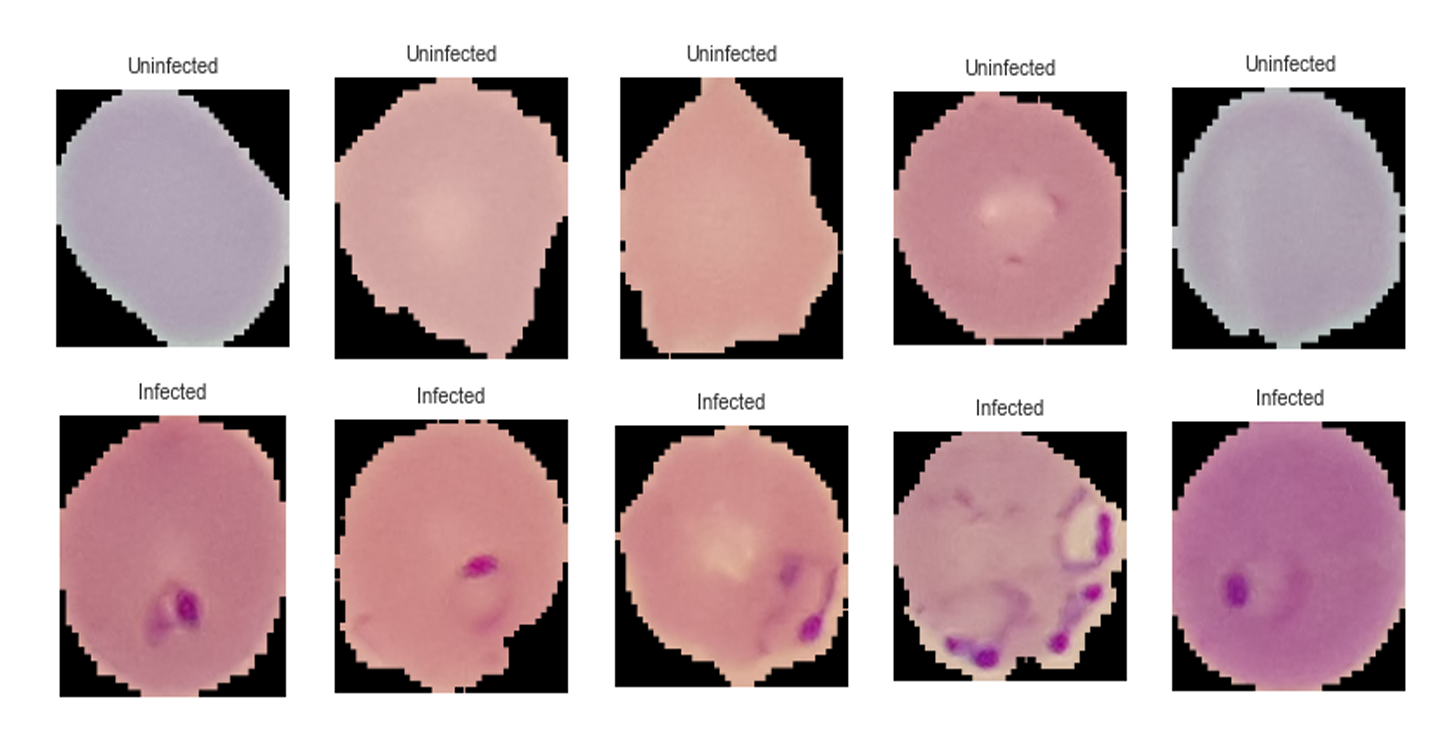
\includegraphics[width=0.8\textwidth]{images/fig1.png}
\caption{Microscopic images from the Dataport dataset showing infected and uninfected cells.}
\label{fig:fig1}
\end{figure}

\begin{figure}[H]
\centering
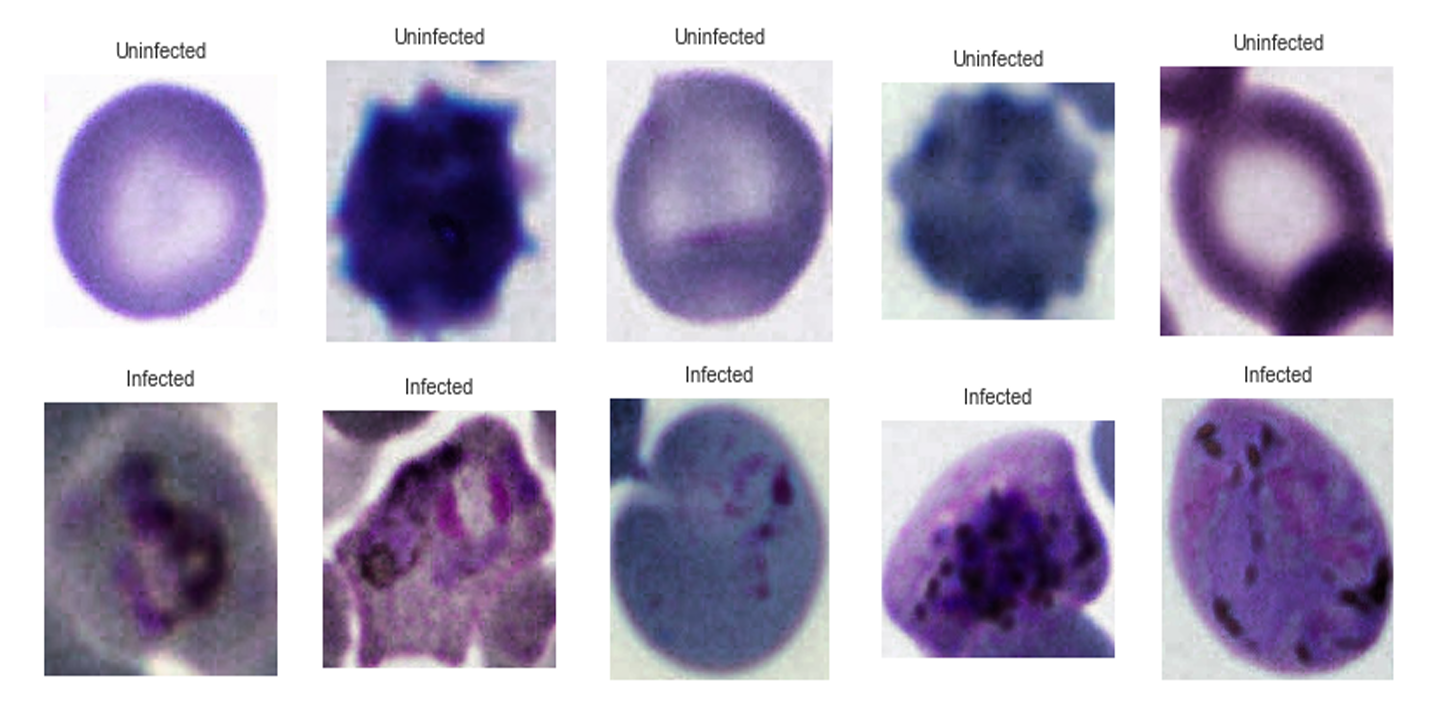
\includegraphics[width=0.8\textwidth]{images/fig2.png}
\caption{Cropped cell images (infected and uninfected) using bounding box annotations from the Kaggle dataset.}
\label{fig:fig2}
\end{figure}

\editornote{(20a) Adjusted figure captions to sentence case to align with IEEE caption style; 
(20b) Reworded captions to more clearly describe the image content and align them with the datasets discussed in the text.}

\section{Proposed Method}
In this research, we propose a one-class convolutional autoencoder designed to learn compressed representations of input images belonging to a single class—specifically, microscopic images of malaria cells. This type of autoencoder is trained to reconstruct its input with minimal error, making it particularly effective for anomaly detection by identifying inputs that deviate significantly from the training distribution.

\editornote{(21a) Rephrased “introduce a novel approach utilizing a one class convolution autoencoder” as “propose a one-class convolutional autoencoder” for clarity and conciseness; 
(21b) Hyphenated “one class” and changed “convolution” to “convolutional” to follow standard ML terminology; 
(21c) Integrated “in this case, microscopic images...” into the main clause using an em dash for smoother flow; 
(21d) Reworded “the unique characteristic... lies in its training objective” as “is trained to reconstruct...” for directness and readability.}

Our proposed autoencoder consists of three main components: an encoder, a latent space, and a decoder. The encoder processes input images—microscopic views of malaria cells—into a lower-dimensional latent representation that captures the most salient features of the data. During training, the autoencoder learns to map normal cell images to a specific region within this latent space, enabling effective differentiation from anomalous inputs.

\editornote{(22a) Merged and restructured overlapping sentences on “latent space” and “essential features” for conciseness and clearer conceptual flow; 
(22b) Reworded “input data, representing the microscopic images...” to “input images—microscopic views of malaria cells” for smoother phrasing; 
(22c) Removed redundant phrasing around “latent space representation” and “encoding”; 
(22d) Recast final sentence to emphasize active learning behavior and clarify the purpose of mapping normal data to a specific region.}

\begin{figure}[H]
\centering
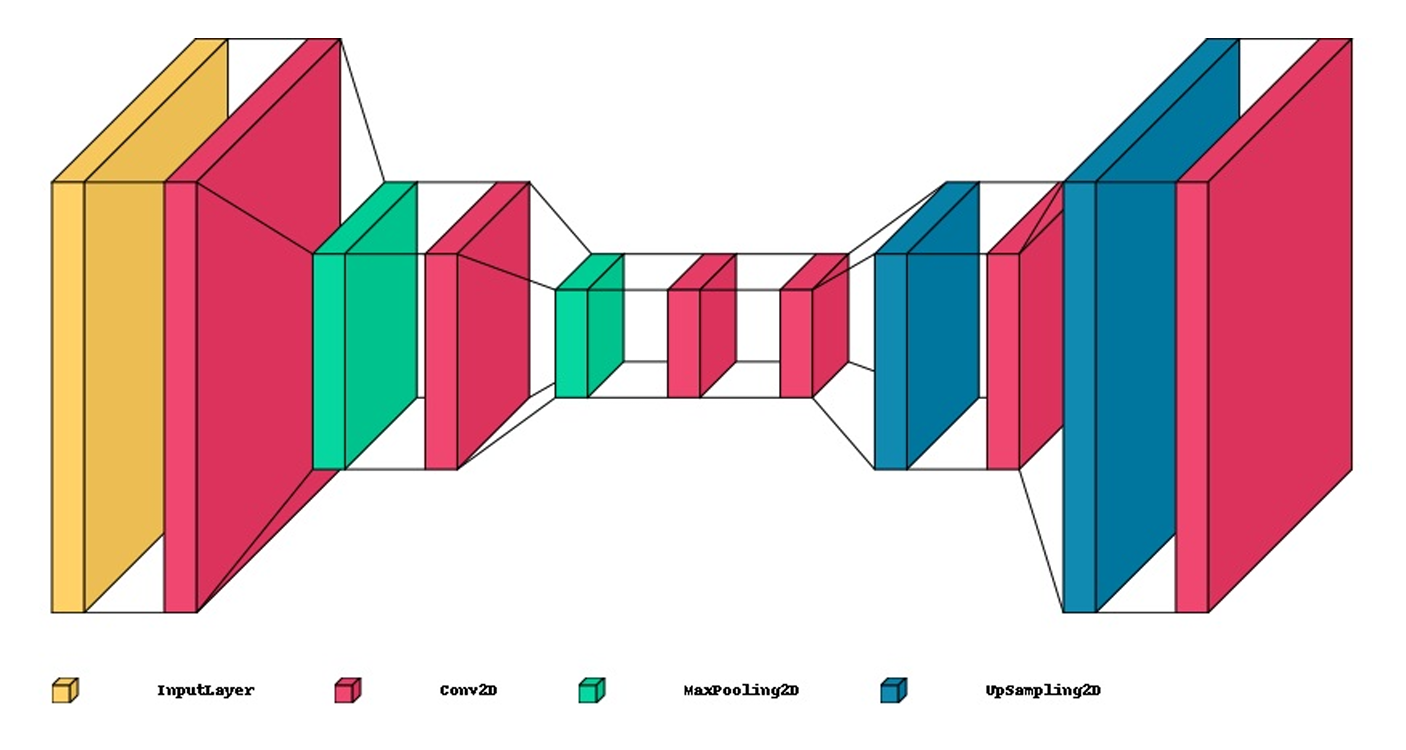
\includegraphics[width=0.8\textwidth]{images/fig3.png}
\caption{Reconstruction of uninfected cell images using an autoencoder.}
\label{fig:fig3}
\end{figure}

\editornote{(23a) Adjusted figure caption to sentence case to conform with IEEE style; 
(23b) Retained original caption structure, but author may consider clarifying whether the figure displays input-output comparison or specific reconstruction quality to enhance interpretability.}

Following the encoder, the decoder attempts to reconstruct the original input from the latent representation. The objective is to generate output that closely resembles the input, completing the reconstruction process. To quantify reconstruction accuracy, we use the mean squared error (MSE) as the loss function:

\begin{equation}
MSE = \frac{1}{N}\sum_{i=1}^{N}(x_i - y_i)^2
\end{equation}

where $N$ represents the total number of samples, $x_i$ is the actual value of the $i$-th sample, and $y_i$ is the predicted value of the $i$-th sample \cite{pu2012}.

\editornote{(24a) Rephrased “Following the encoder, the decoder, the second part of the network...” as “Following the encoder, the decoder...” to reduce redundancy and clarify subject; 
(24b) Reworded “generate output that closely resembles...” to “reconstruct the original input...” for conciseness and technical accuracy; 
(24c) Simplified “To quantify the quality of this reconstruction...” to “To quantify reconstruction accuracy...” for clarity.}

The model is trained to minimize this loss, encouraging the reconstructed outputs to closely match the original inputs.

\editornote{(25a) Replaced “aims to minimize” with “is trained to minimize” for clarity;
(25b) Reworded “ensuring that the reconstructed outputs align...” as “encouraging the reconstructed outputs to closely match...” to improve clarity.}

During training, the one-class autoencoder is exposed exclusively to normal, non-anomalous data. It learns to accurately reconstruct these inputs, and the latent space is shaped by their distribution. As a result, the model becomes effective at capturing the characteristic patterns of normal cell images.

\editornote{(26a) Removed “It is important to note that...” to maintain direct academic tone; 
(26b) Reduced repetition of “normal data” by varying phrasing (“these inputs,” “normal cell images”); 
(26c) Recast “latent space representations are shaped...” as “the latent space is shaped by their distribution” for clarity and active structure; 
(26d) Reworded “becomes adept at capturing” as “becomes effective at capturing” for formality.}

We use the Structural Similarity Index (SSIM) to evaluate the similarity between original and reconstructed images. During testing, SSIM provides a quantitative measure of how closely reconstructed images of unknown samples match the distribution of known class data. Higher SSIM scores indicate a stronger resemblance, offering insight into the quality of the model’s reconstructions \cite{fu2017}.

\editornote{(27a) Replaced “As a means of evaluation, we utilize...” with “We use...” to improve clarity and conciseness; 
(27b) Reworded “enabling an understanding of the similarity...” as “to evaluate the similarity...” for directness; 
(27c) Clarified phrasing of “unknown class samples and known class data” to emphasize comparative structure; 
(27d) Consolidated repeated mentions of similarity and reconstruction quality to streamline flow.}

According to Wang et al. \cite{wang2009}, the SSIM methodology is based on the principle that the human visual system is especially sensitive to structural information in visual scenes. Preserving this structural detail is therefore essential when assessing image fidelity. SSIM differentiates between two types of distortions: nonstructural and structural. Nonstructural distortions—such as changes in luminance, contrast, gamma, or spatial alignment—typically result from environmental or instrumental factors and do not alter the underlying structure of visual objects. In contrast, structural distortions, including additive noise, blur, and lossy compression, directly degrade the spatial organization of object features within an image.

\editornote{(28a) Added comma after “Wang et al. \cite{wang2009}” for correct introductory clause punctuation; 
(28b) Rephrased “rooted in the understanding that...” as “based on the principle that...” for conciseness and flow; 
(28c) Improved clarity and structure of the distinction between nonstructural and structural distortions; 
(28d) Reorganized distortion lists for balance and readability; grouped similar items and clarified causal phrasing (e.g., “result from environmental or instrumental factors”); 
(28e) Strengthened final contrast between distortion types with more parallel sentence construction.}

The SSIM framework is inspired by the human visual system, which is modeled as an ideal information extractor capable of recognizing objects under various types of distortion. Accordingly, SSIM emphasizes sensitivity to structural distortions while compensating for nonstructural ones. The index operates on local image patches (denoted as $x$ and $y$) from two compared images. It evaluates similarity based on three components: luminance $l(x, y)$, contrast $c(x, y)$, and structural correlation $s(x, y)$. These components are computed using simple statistical measures and then combined to produce a local SSIM score, $S(x, y)$.

\editornote{(29a) Rephrased “takes inspiration from the human visual system” as “is inspired by the human visual system” for formality and clarity; 
(29b) Clarified “amidst various distortions” to “under various types of distortion” for precision; 
(29c) Recast “easily computed statistics” as “simple statistical measures” to maintain objective tone; 
(29d) Smoothed sentence structure around notational elements $l(x, y)$, $c(x, y)$, $s(x, y)$, and $S(x, y)$ for better readability and parallelism.}

The SSIM formula is composed of interpretable components that quantify luminance, contrast, and structural similarity between image patches:

\begin{equation}
SSIM(x, y) = \frac{(2\mu_x\mu_y + C_1)(2\sigma_{xy} + C_2)}{(\mu_x^2 + \mu_y^2 + C_1)(\sigma_x^2 + \sigma_y^2 + C_2)}
\end{equation}

Here, $\mu_x$ and $\mu_y$ are the local means of patches $x$ and $y$, $\sigma_x$ and $\sigma_y$ are the corresponding standard deviations, and $\sigma_{xy}$ is the cross-covariance between $x$ and $y$. The constants $C_1$ and $C_2$ are small positive values introduced to stabilize the division when denominators are close to zero.

\editornote{(30a) Reworded “while seemingly complex, breaks down into manageable components” as “is composed of interpretable components” to maintain objective and confident tone; 
(30b) Corrected the SSIM formula structure by using proper multiplicative grouping (note original used a plus sign between terms in numerator, which is likely a transcription error? I believe the original SSIM use multiplication); 
(30c) Removed $C_3$, which does not appear in this equation and is unnecessary unless referenced elsewhere; 
(30d) Clarified variable definitions using parallel structure and improved terminology (e.g., “cross-covariance” instead of “sample cross-correlation”).}

The SSIM index exhibits symmetry ($S(x, y) = S(y, x)$) and is bounded within the range of -1 to 1. A score of 1 indicates perfect similarity between the compared patches. The index operates within a sliding window, yielding an SSIM map, and the overall image SSIM score is computed—often by averaging SSIM values across the image. Adaptive space-variant weighting and scale-based computations enhance its performance across various spatial scales.

\editornote{(31a) Formatted “S(x, y) = S(y, x)” in math mode, as I had neglected to do so during my original transcription efforts; 
(31b) Corrected “a SSIM map” to “an SSIM map”; 
(31c) Rephrased “yielding a SSIM map... averaging SSIM values” to improve flow and sentence balance.}

In our approach, classification is based on a predefined SSIM threshold, which is selected according to an acceptable false negative rate (FNR) specified by the practitioner. This threshold is determined using the validation set and the autoencoder’s reconstructed images. A histogram is generated to compare SSIM-based reconstruction errors for normal and anomalous validation samples. We then select a threshold such that most normal images exhibit reconstruction errors above this value, maximizing the model’s ability to distinguish normal from anomalous inputs.

\editornote{(32a) Rephrased passive “classification decisions are made…” to active “classification is based on…” for conciseness; 
(32b) Clarified that the FNR is specified by the user/practitioner; 
(32c) Reworded “we plot a bar graph” to “a histogram is generated” for formality; 
(32d) Smoothed the threshold selection explanation to clarify that the threshold is set so that most normal images are above it in terms of SSIM error—though this logic may need verification, as lower SSIM usually indicates poorer reconstruction. Recommend reviewing the figure referenced here to confirm error polarity.}

For each test sample, a reconstruction error based on SSIM is computed. If this error exceeds the predefined threshold, the sample is classified as belonging to the normal class. Conversely, samples with errors below the threshold are considered anomalous. This approach provides a principled decision boundary, enhancing the reliability of the classification process.

\editornote{(33a) Rephrased “its SSIM-based reconstruction error is calculated” for more fluid sentence structure; 
(33b) Clarified threshold logic using more concise phrasing and removed minor repetition; 
(33c) Replaced “statistically significant criterion” with “principled decision boundary” for greater clarity and technical precision.}

Accordingly, using a predefined threshold \( \varepsilon \), test samples are classified according to the following decision rule:

\begin{equation}
x_t \in \begin{cases} 
\text{known class,} & \text{if } \varepsilon_t < \varepsilon \\
\text{unknown class,} & \text{otherwise}
\end{cases}
\end{equation}

The threshold \( \varepsilon \) is typically determined by the user based on an acceptable false negative rate (FNR).

\editornote{(34a) Replaced “Correspondingly” with “Accordingly” for smoother transitional phrasing; 
(34b) Reworded “can be discriminated by” as “are classified according to the following decision rule” for clarity; 
(34c) Removed “Note that...” to maintain formal tone and began final sentence directly with “The threshold...”.}

In summary, our proposed method employs a one-class autoencoder trained to reconstruct normal microscopic images of malaria cells. This enables the model to identify anomalous or infected instances during testing, demonstrating its potential to improve the accuracy of malaria diagnosis.

\begin{figure}[H]
\centering
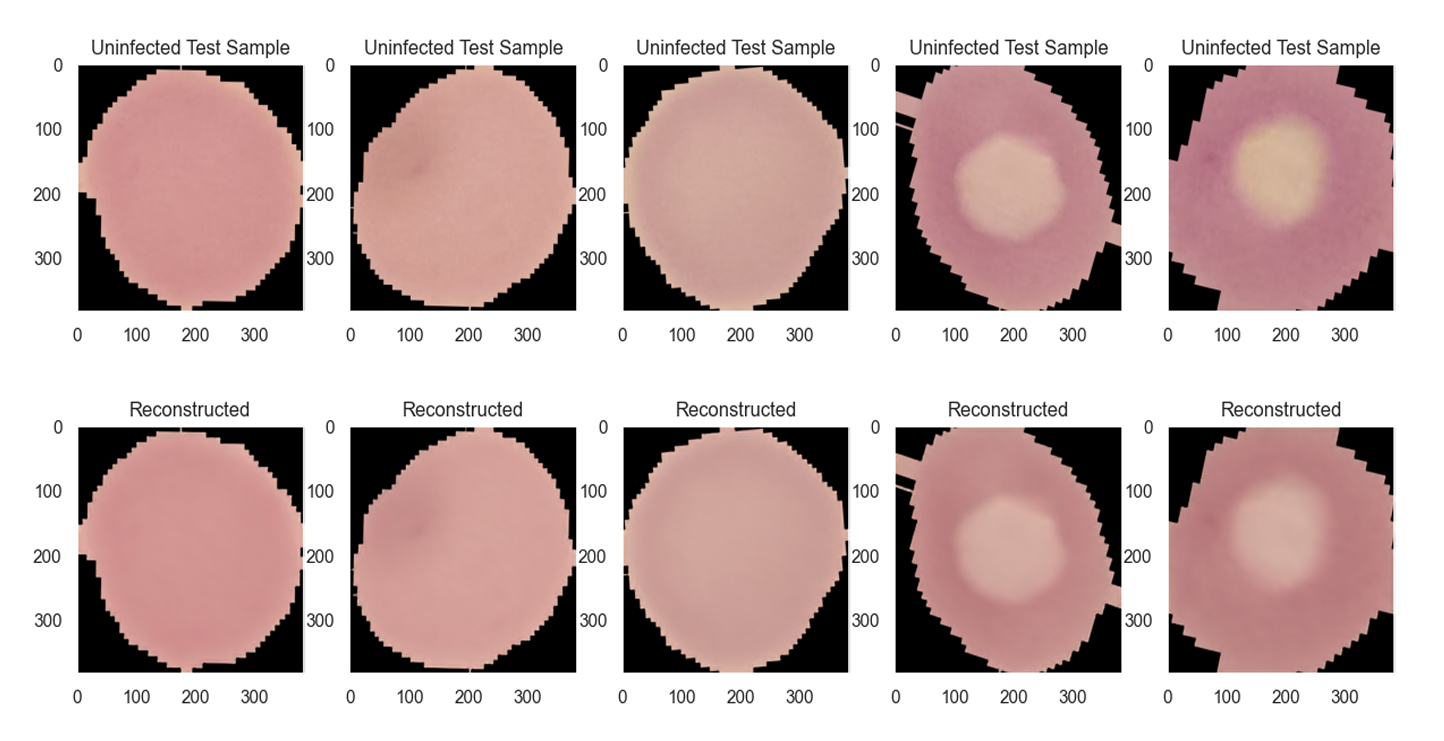
\includegraphics[width=0.8\textwidth]{images/fig4.png}
\caption{Reconstruction of uninfected cell images from the IEEE Dataport dataset using an autoencoder.}
\label{fig:fig4}
\end{figure}

\editornote{(35a) Replaced “leverages the power of” with “employs” for a more objective and direct tone; 
(35b) Removed redundant phrasing “learn and reconstruct” in favor of “trained to reconstruct”; 
(35c) Streamlined “Through this approach, we enable the model to...” as “This enables the model to...” to improve sentence flow; 
(35d) Reworded “showcasing the potential of our method in enhancing” as “demonstrating its potential to improve” for conciseness and clarity.
(35e) Adjusted figure caption to sentence case to align with IEEE style guidelines; rephrased for clarity by specifying “uninfected cell images from the IEEE Dataport dataset” rather than using redundant or ambiguous phrasing (“Dataport IEEE Dataset Uninfected Cell Images”).}

\section{Results}
To assess the effectiveness of our proposed method, we evaluated the model using several performance metrics that quantify accuracy and classification quality:

\begin{figure}[H]
\centering
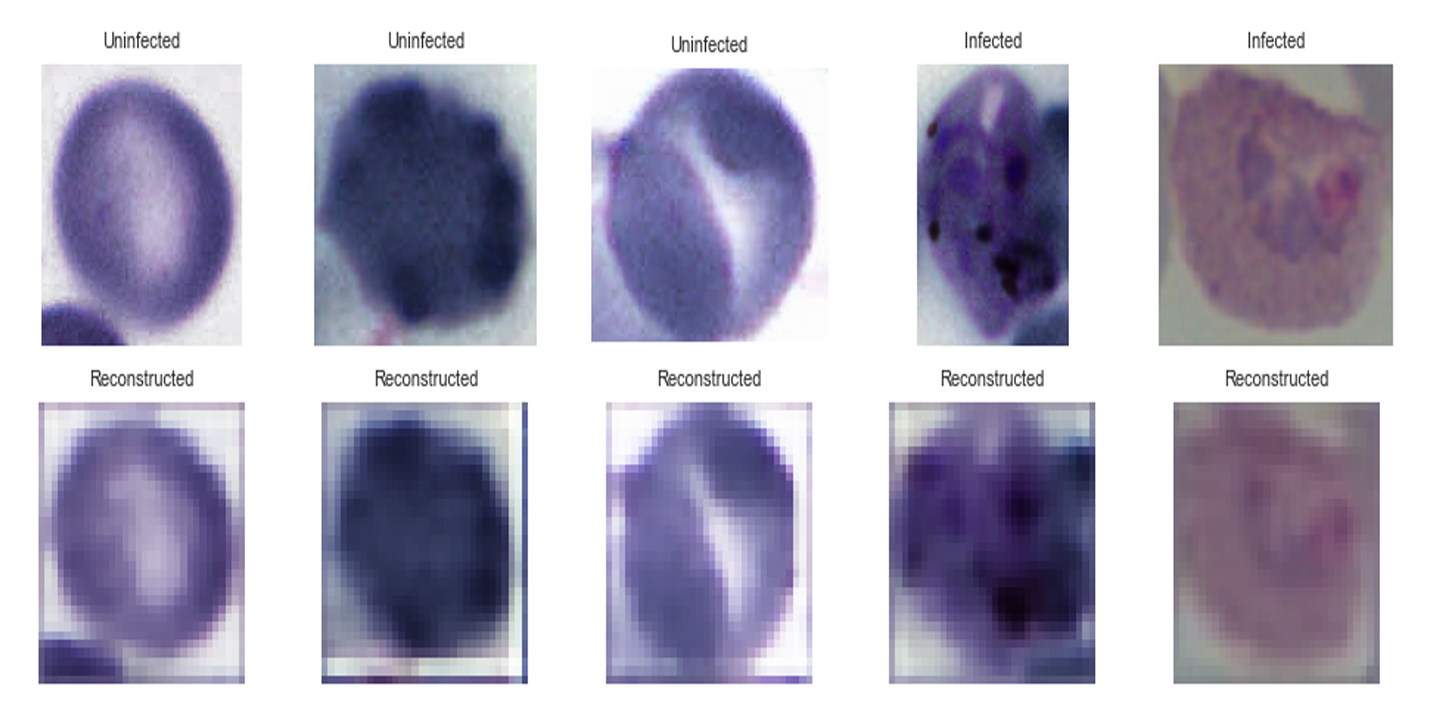
\includegraphics[width=0.8\textwidth]{images/fig5.png}
\caption{Reconstruction of cell images from the Kaggle bounding box dataset using an autoencoder.}
\label{fig:fig5}
\end{figure}

\editornote{(36a) Rephrased “Evaluating the viability of our proposed method is an essential part...” as “To assess the effectiveness of our proposed method...” for conciseness and specificity;
(36b) Reworded “Metrics are used to evaluate... and to understand...” as “we evaluated the model using several performance metrics...” to eliminate redundancy;
(36c) Clarified the metric purpose (accuracy and classification quality) for better context;
(36d) Adjusted figure caption to sentence case and clarified that the dataset shown is the Kaggle bounding box dataset, aligning with prior dataset references.}

SSIM was selected as an evaluation metric because it captures both global and local features in reconstructed images, emphasizing perceptual similarity. This makes it well-suited for assessing how effectively the model preserves critical visual structure. Integrating SSIM with thresholding improves the method’s precision and robustness when classifying malaria-infected cells in microscopic images, supporting its utility in medical diagnostics.

\editornote{(37a) Replaced “Leveraging SSIM as an evaluation metric aligns with our goal...” with a more concise rationale: “SSIM was selected... because it captures...”;
(37b) Combined overlapping ideas around “perceptual similarity” and “preserve critical visual information” to improve cohesion and reduce redundancy;
(37c) Reworded “enhances the precision and reliability... making it a robust tool for accurate medical diagnosis and analysis” as “improves the method’s precision and robustness... supporting its utility in medical diagnostics” to streamline phrasing and avoid repetition of “accurate” and “robust.”}

To determine the most effective evaluation metric for distinguishing normal and abnormal cell images, we compared mean squared error (MSE) and structural similarity index (SSIM). Our goal was to identify a metric that supports high classification accuracy while minimizing false positive rates.

\editornote{(38a) Replaced “Our attention was drawn towards comparing and identifying a useful evaluation metric...” with “To determine the most effective evaluation metric...” for clarity and conciseness; 
(38b) Separated the long sentence into two for better readability and emphasis; 
(38c) Rephrased “with high accuracy and a very low false positive rate” as “supports high classification accuracy while minimizing false positive rates” to improve rhythm and align with technical tone.}

MSE performed poorly in classifying malaria cell images. This limitation is well documented in the work of Wang et al. \cite{wang2009}, who demonstrated the shortcomings of MSE and the advantages of SSIM as an image evaluation metric.

\editornote{(39a) Replaced “gave very poor results when it comes to...” with “performed poorly in classifying...” for grammatical correctness and formal tone;
(39b) Rephrased “this was evidenced by the research done by Wang et al... who illustrated...” as “This limitation is well documented in the work of Wang et al., who demonstrated...” for conciseness and flow;
(39c) Corrected spelling of “metris” to “metrics” and clarified the comparison being made.}

According to Wang et al. \cite{wang2009}, mean squared error (MSE), while effective as a loss function, has several limitations when used as an image evaluation metric.

\textbf{Lack of Sensitivity to Human Perception:} MSE does not reflect how humans perceive visual differences. It treats all pixel errors equally, ignoring that some discrepancies are more perceptually significant than others. For example, small errors in smooth regions may go unnoticed, while similar errors in textured or high-contrast areas are more apparent. This failure to account for perceptual salience leads to inaccurate assessments of image quality.

\editornote{(40a) Added comma after citation for proper syntax: “Wang et al. \cite{wang2009}, MSE...”;
(40b) Split the opening sentence into two for readability and to better distinguish MSE’s use as a loss function versus evaluation metric;
(40c) Replaced “various setbacks as follows” with “several limitations” for modern and concise tone;
(40d) Reworded “how humans perceive differences in visual perception” as “how humans perceive visual differences” to eliminate redundancy;
(40e) Clarified phrasing in the example sentence for rhythm and flow.}

\textbf{Inability to capture structural information:} Images contain structural elements—such as edges, textures, and spatial patterns—that are crucial for human perception. MSE treats images as collections of independent pixels and fails to account for spatial relationships among features. Even when pixel values remain constant, changes in these relationships can significantly affect perceived image quality.

\editornote{(41a) Changed heading to sentence case (“Inability to capture structural information”) to match formatting style used in earlier list items;
(41b) Rephrased “images often contain structural elements such as...” as “images contain structural elements—such as...” for improved flow;
(41c) Recast “collection of independent pixels” and “fails to capture these structural relationships” to more technically precise phrasing;
(41d) Clarified the final sentence by specifying that perceptual changes occur due to changes in spatial relationships, not just raw values.}

\textbf{Failure to address image content-dependent variations:} MSE treats all pixels equally, regardless of their perceptual relevance. In many images, certain regions—such as faces in portraits—carry greater visual significance than others. This uniform weighting prevents MSE from accounting for differences in how viewers prioritize visual information.

\editornote{(42a) Converted heading to sentence case for consistency with previous list items;
(42b) Replaced repeated “perceptual importance” with “perceptual relevance” and “visual significance” to improve lexical variety;
(42c) Reworded final sentence to avoid passive phrasing and improve clarity around what MSE fails to account for.}

\textbf{Neglect of error signal characteristics:} MSE does not account for the structure of the error signal, such as its correlation with the original image or the sign (positive or negative) of pixel-wise errors. In real-world scenarios, these errors are often content-dependent, and their directionality can influence visual perception. MSE’s uniform treatment of all deviations overlooks these important perceptual factors.

\editornote{(43a) Adjusted heading to sentence case for consistency with previous critiques;
(43b) Rephrased “such as its correlation with the original image or the signs of error signal samples” to “such as its correlation... or the sign (positive or negative) of pixel-wise errors” for clarity and conciseness;
(43c) Reworded final sentence to improve flow and emphasize perceptual implications.}

These limitations of MSE are addressed by SSIM, which evaluates image quality using perceptual principles. Its assessment considers structural and statistical features that align more closely with human visual perception. SSIM evaluates images based on three components:

\textbf{Luminance comparison:} SSIM computes the luminance term by comparing the average pixel intensities of two images. This reflects how the overall brightness of the images corresponds. When the average intensities are similar, it indicates similarity in luminance.

\editornote{(44a) Replaced “These characteristics are towered by the efficient ways that SSIM sees, perceives and evalutes images...” with “These limitations of MSE are addressed by SSIM, which evaluates image quality using perceptual principles...” for clarity, tone, and grammar;
(44b) Corrected spelling of “evalutes” and removed informal verbs (“sees” and “perceives”) in favor of more technical phrasing;
(44c) Formatted “Luminance Comparison” to sentence case to match previous list styles;
(44d) Removed redundant phrasing in the final sentence for conciseness and improved flow.}

\textbf{Contrast comparison:} The contrast term is calculated by comparing the standard deviations of pixel intensities in each image, which reflects the degree of local variation. Images with similar contrast will exhibit small differences in these standard deviations, indicating a close match in contrast characteristics.

\editornote{(45a) Changed heading to sentence case (“Contrast comparison”) to maintain consistency with previous items;
(45b) Combined first two sentences for better flow and to reduce redundancy;
(45c) Rephrased final sentence to avoid repetition of “contrast” and to clarify how similarity is inferred from standard deviation values.}

\textbf{Structure comparison:} The structure term measures the correlation between corresponding pixels in the two images, capturing the spatial relationships that define structural similarity. When pixel intensities are strongly correlated in aligned regions, this indicates similar structural organization between the images.

\editornote{(46a) Changed heading to sentence case (“Structure comparison”) for consistency;
(46b) Rephrased “correlation between pixel intensities of the images” to “correlation between corresponding pixels” for clarity and conciseness;
(46c) Reworded final sentence to improve rhythm and avoid repetitive phrasing (“correlated...correlation...similarity”).}

These principles made SSIM the most effective evaluation metric for this task. We evaluated our model using several standard classification metrics:

\textbf{Accuracy:} This metric measures the proportion of correct predictions made by the model. Values closer to 1.0 (or 100\%) indicate stronger overall performance \cite{powers2011}.

\editornote{(47a) Rephrased “the best placed method as an evaluation metric” as “the most effective evaluation metric for this task” to improve clarity and formality;
(47b) Corrected spelling of “evaluted” to “evaluated”;
(47c) Added colon after transitional sentence to introduce the metric list properly;
(47d) Combined two repetitive statements in the “Accuracy” bullet into one concise explanation.}

\textbf{Recall:} Also known as sensitivity or true positive rate, recall measures a model’s ability to correctly identify all relevant instances—in this case, malaria-infected cells. Missing an infected cell (a false negative) may have serious medical consequences, so maximizing recall for the positive class is critical \cite{powers2011}.

\editornote{(48a) Lowercased “Recall” in the heading to maintain sentence case formatting;
(48b) Streamlined definition of recall to reduce redundancy and improve parallel structure with previous metrics;
(48c) Condensed the medical rationale into a single, high-impact sentence emphasizing the consequence of false negatives.}

\textbf{Precision:} Precision measures how many of the instances predicted as positive by the model are actually correct. It quantifies the proportion of true positives among all predicted positives \cite{powers2011}.

\editornote{(49a) Lowercased “Precision” in the heading for consistency with previous metric entries;
(49b) Rephrased “positive predictions made by the model” to “instances predicted as positive by the model” for smoother flow;
(49c) Consolidated phrasing to avoid redundancy while maintaining clarity in distinguishing true vs. predicted positives.}

\textbf{F1 score:} The F1 score is the harmonic mean of precision and recall, providing a single value that balances both metrics. It is especially useful when there is a trade-off between false positives and false negatives, as it captures both the completeness and exactness of the model’s predictions \cite{powers2011}.

\editornote{(50a) Lowercased “F1 Score” to “F1 score” in heading to match list style;
(50b) Removed repeated definitions of precision and recall, since they were just introduced above;
(50c) Clarified that F1 is useful when both types of classification error (false positives and false negatives) matter.}

\textbf{Specificity:} Specificity measures the proportion of actual negative instances (e.g., non-infected cells) that the model correctly identifies. It reflects the model’s ability to avoid false positives by accurately classifying negative cases \cite{powers2011}.

\editornote{(51a) Maintained sentence case for “Specificity” heading for consistency; 
(51b) Removed redundant phrasing in “correctly identifies as negative” and “correctly classifying negative instances” to streamline explanation;
(51c) Reworded second sentence to avoid repetition and clarify the metric’s purpose in terms of false positives.}

\subsection{Evaluation Metrics Results}
While the autoencoder did not yield optimal results initially, it effectively minimized loss over the 35 training epochs. The consistent decrease in both training and validation loss indicates successful compression of input data while preserving essential features. Moreover, the absence of divergence between training and validation losses suggests stable learning without signs of overfitting. These outcomes provide a solid foundation for future refinement of the model.

\editornote{(52a) Rephrased “although not delivering optimal results initially” as “did not yield optimal results initially” for conciseness and clarity;
(52b) Condensed “training period spanning 35 epochs” to “over the 35 training epochs” to reduce verbosity;
(52c) Smoothed phrasing around loss trend to eliminate redundancy (e.g., “signifies the model’s ability...” → “indicates...”);
(52d) Replaced passive and padded constructions like “this outcome indicates...” with more direct equivalents;
(52e) Reworded final sentence for improved structure and stronger closure.}

The confusion matrix analysis revealed limitations with the mean squared error (MSE) metric. Specifically, the MSE-based model struggled to distinguish accurately between infected and uninfected cells, exhibiting elevated rates of both false positives and false negatives. As shown in the confusion matrices, this performance reflects MSE’s inability to capture the subtle visual patterns critical for malaria detection. In contrast, the structural similarity index (SSIM)—which incorporates luminance, contrast, and structural features—more effectively captured image-level distinctions. As a result, models evaluated with SSIM demonstrated greater classification accuracy and reliability, making it the more suitable metric for this task.

\editornote{(53a) Replaced “the MSE-based” with “the MSE-based model” to correct incomplete phrasing;
(53b) Reworded “highlighted some challenges” and “struggled in accurately distinguishing...” for conciseness and grammar;
(53c) Smoothed transitions between MSE and SSIM descriptions to maintain parallel structure;
(53d) Replaced “more adept at capturing” with “more effectively captured” for tone consistency;
(53e) Recast final sentence to emphasize SSIM’s demonstrated performance without repetition of “this shows that...”}

The model demonstrated strong performance across both the Bounding Boxes Kaggle Malaria dataset and the IEEE Dataport Malaria Dataset. It achieved a recall of 0.97 on the Kaggle dataset and 0.99 on the IEEE dataset, indicating a high true positive rate in identifying malaria-infected cells. These results highlight the model’s effectiveness in detecting abnormal instances and provide a basis for further refinement.

\editornote{(54a) Replaced subjective phrases like “exceptional results,” “outstanding performance,” and “remarkable true positive rate” with more neutral, descriptive language (e.g., “strong performance” and “high true positive rate”);
(54b) Removed promotional phrasing such as “instill confidence” and “inspire optimism”;
(54c) Combined redundant phrases to tighten flow and emphasize the key numerical results;
(54d) Maintained clarity around dataset names and performance metrics for accurate attribution.}

\begin{figure}[H]
  \centering
  \begin{minipage}{0.45\textwidth}
    \centering
    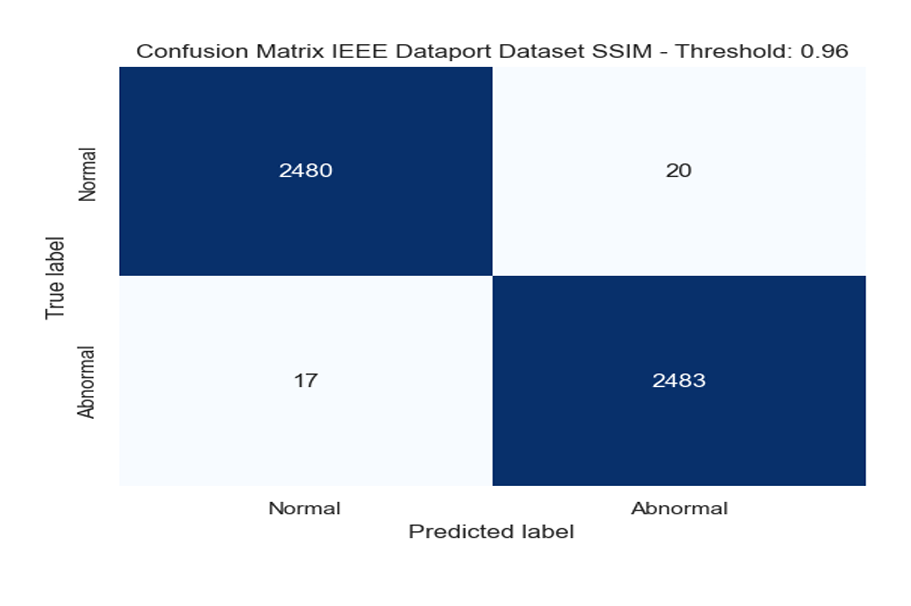
\includegraphics[width=\textwidth]{images/fig6.png}
    \caption{Confusion matrix (SSIM, threshold = 0.96).}
    \label{fig:fig6}
  \end{minipage}\hfill
  \begin{minipage}{0.45\textwidth}
    \centering
    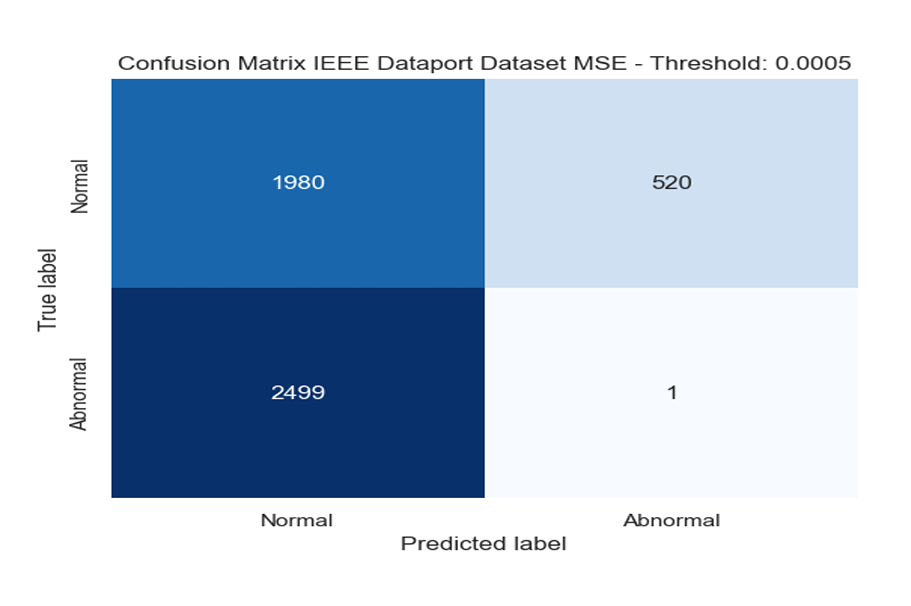
\includegraphics[width=\textwidth]{images/fig7.png}
    \caption{Confusion matrix (MSE, threshold = 0.0015).}
    \label{fig:fig7}
  \end{minipage}
\end{figure}

\editornote{
(55a) Corrected caption style to IEEE sentence case (“Confusion matrix” instead of “Confusion Matrix”);
(55b) Standardized metric references in parentheses with lowercase abbreviations and fixed spacing (e.g., “(SSIM, threshold = 0.96)”);
(55c) Added equals sign in threshold formatting (“threshold = 0.96” rather than appositive phrasing);
(55d) Added ending period to both captions to match IEEE caption punctuation standards.}

  
\begin{figure}[H]
  \centering
  \begin{minipage}{0.45\textwidth}
    \centering
    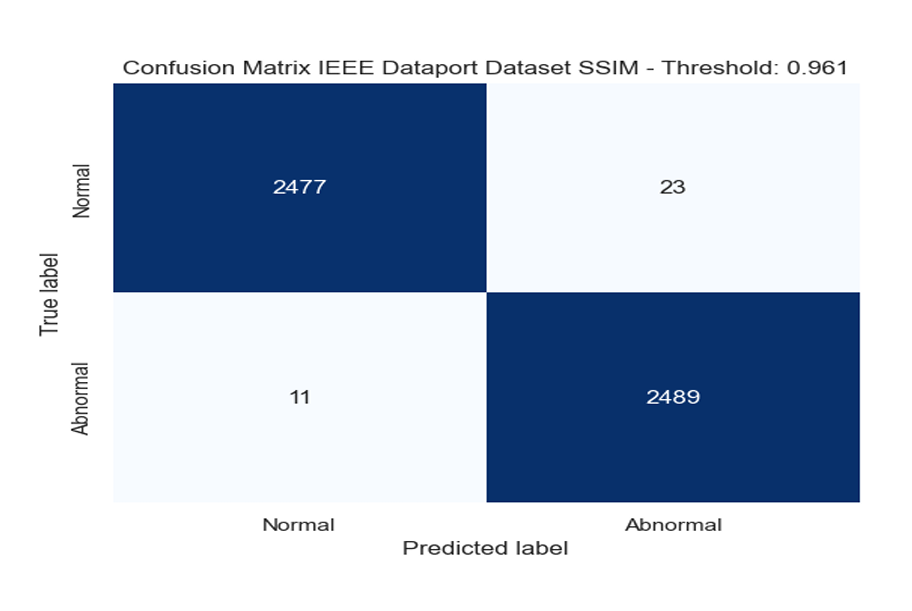
\includegraphics[width=\textwidth]{images/fig8.png}
    \caption{Confusion matrix (SSIM, threshold = 0.961).}
    \label{fig:fig8}
  \end{minipage}\hfill
  \begin{minipage}{0.45\textwidth}
    \centering
    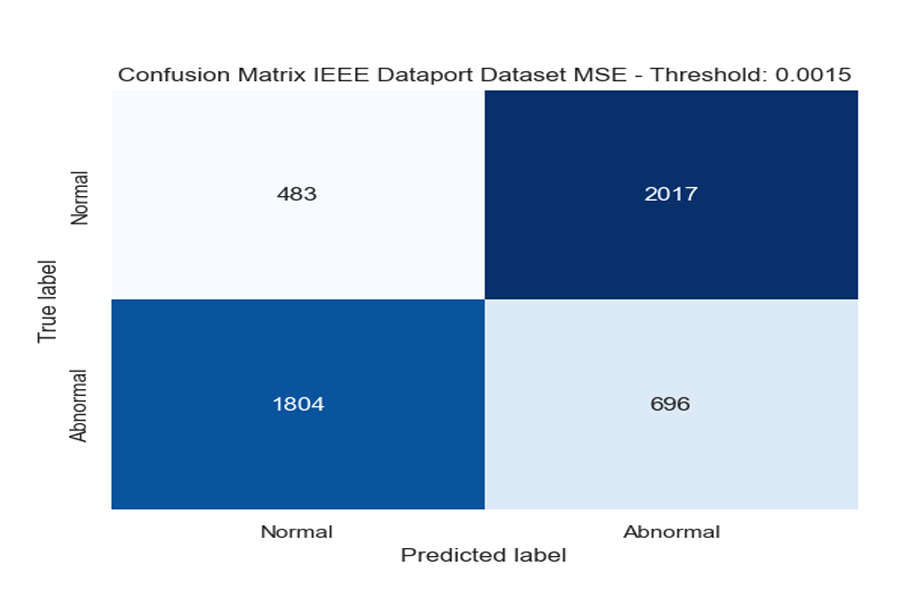
\includegraphics[width=\textwidth]{images/fig9.png}
    \caption{Confusion matrix (MSE, threshold = 0.0025).}
    \label{fig:fig9}
  \end{minipage}
\end{figure}

\editornote{
(56a) Reformatted both captions to IEEE sentence case (e.g., “Confusion matrix”);
(56b) Added parentheses and standardized formatting for metric and threshold (e.g., “(SSIM, threshold = 0.961)”);
(56c) Ensured consistent punctuation and spacing across captions;
(56d) Added final periods to both captions to meet IEEE caption punctuation standards.}

  
\begin{figure}[H]
  \centering
  \begin{minipage}{0.45\textwidth}
    \centering
    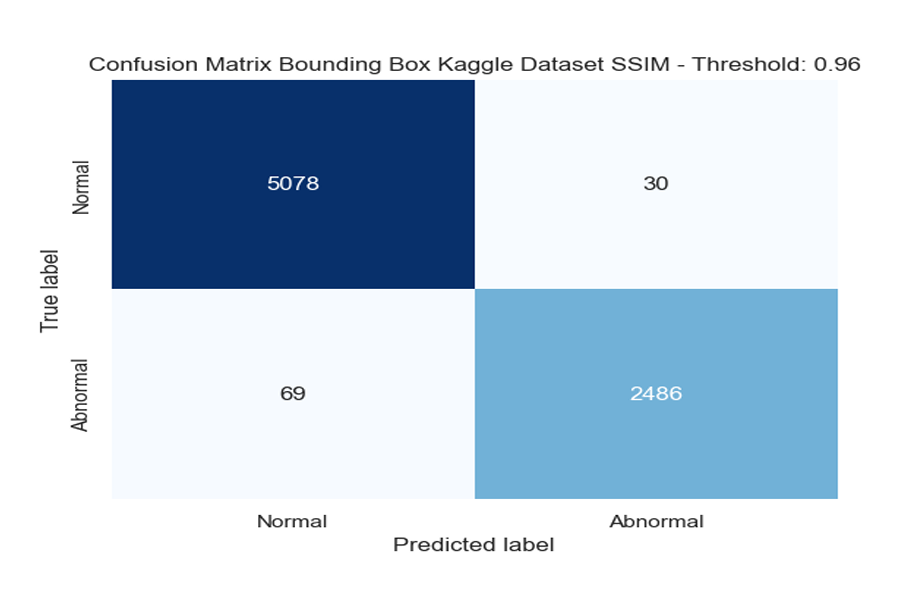
\includegraphics[width=\textwidth]{images/fig10.png}
    \caption{Confusion matrix (SSIM, threshold = 0.96).}
    \label{fig:fig10}
  \end{minipage}\hfill
  \begin{minipage}{0.45\textwidth}
    \centering
    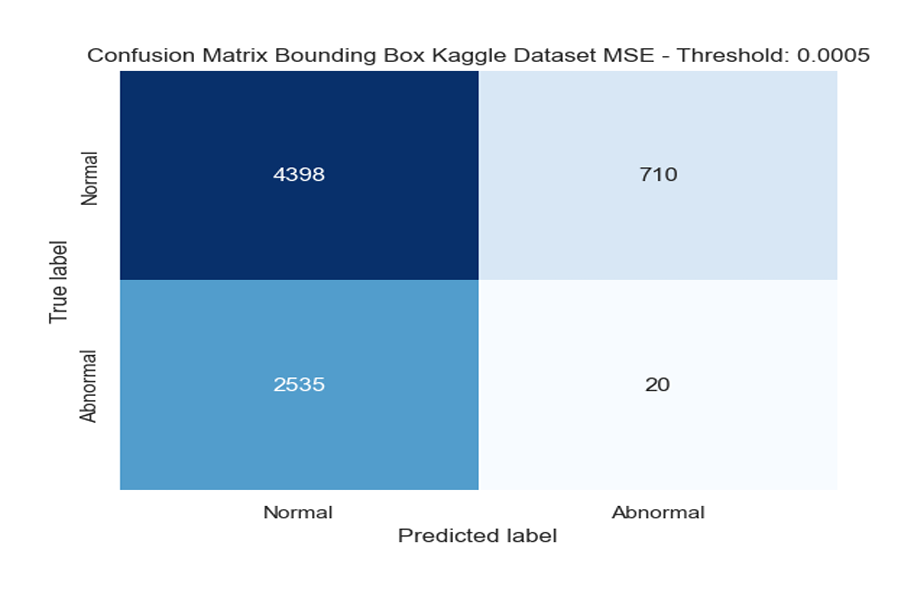
\includegraphics[width=\textwidth]{images/fig11.png}
    \caption{Confusion matrix (MSE, threshold = 0.0035).}
    \label{fig:fig11}
  \end{minipage}
\end{figure}

\editornote{
(57a) Reformatted both figure captions to use sentence case and metric-first naming (e.g., “Confusion matrix (SSIM, threshold = 0.96)”); 
(57b) Added parentheses around metric/threshold and standardized spacing; 
(57c) Appended periods to match IEEE caption punctuation rules.}
  
\begin{figure}[H]
  \centering
  \begin{minipage}{0.45\textwidth}
    \centering
    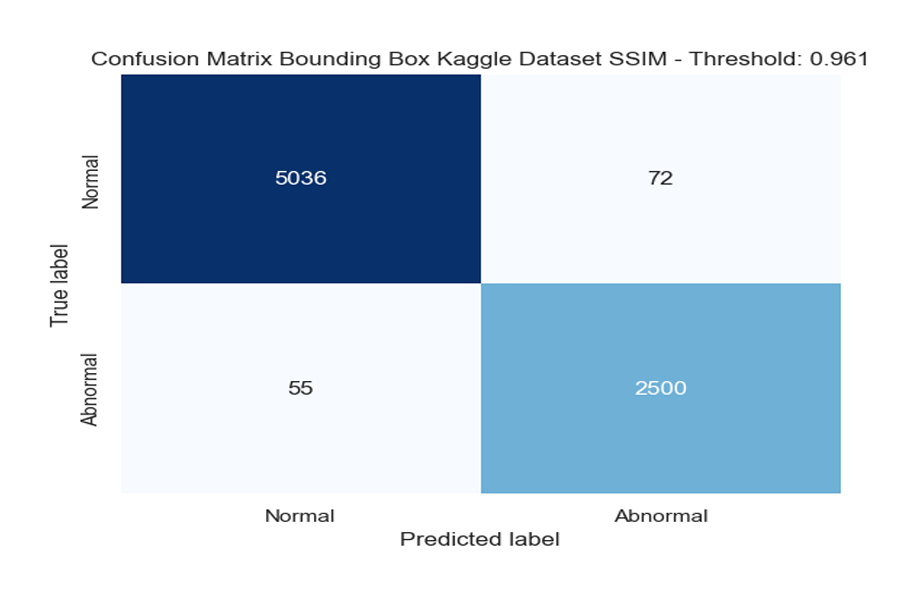
\includegraphics[width=\textwidth]{images/fig12.png}
    \caption{Confusion matrix (SSIM, threshold = 0.961).}
    \label{fig:fig12}
  \end{minipage}\hfill
  \begin{minipage}{0.45\textwidth}
    \centering
    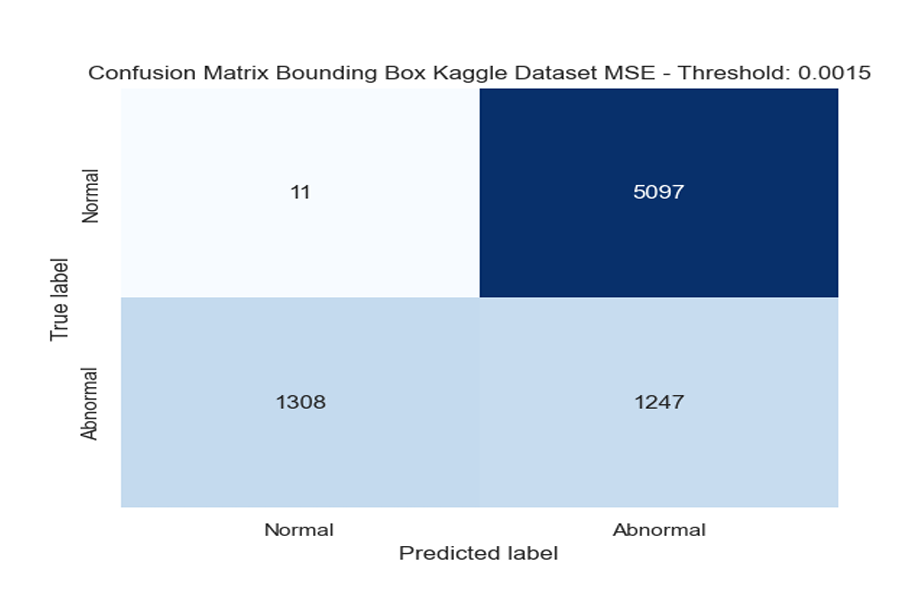
\includegraphics[width=\textwidth]{images/fig13.png}
    \caption{Confusion matrix (MSE, threshold = 0.0045).}
    \label{fig:fig13}
\end{minipage}
\end{figure}

\editornote{
(58a) Revised caption for Figure 12 to follow sentence case and IEEE caption style: “Confusion matrix (SSIM, threshold = 0.961).”;
(58b) Standardized punctuation and format for metric-labeling consistency across all confusion matrix figures.
}

\editornote{
(59a) Edited caption for Figure 13 to match standardized format: “Confusion matrix (MSE, threshold = 0.0045).”;
(59b) Applied sentence case and reordered elements for clarity and IEEE style compliance; matches format used in previous confusion matrix figures.
}
  
\begin{figure}[H]
  \centering
  
\includegraphics[width=\textwidth]{images/fig14.png}
  \caption{Placeholder: Combined SSIM and MSE confusion matrices (figure pending).}
  \label{fig:fig14}
\end{figure}

\editornote{
(60a) Noted that Figure 14 is currently a placeholder image due to missing source content;
(60b) Updated the caption to: “Placeholder: Combined SSIM and MSE confusion matrices (figure pending)” to accurately reflect the current state of the image and prevent misinterpretation by reviewers.
}

The precision of 0.99 for both datasets demonstrates the model's strong performance in identifying positive cases. Notably, the recall for abnormal instances is also high—0.97 for the Bounding Boxes Kaggle Malaria dataset and 0.99 for the IEEE Dataport Malaria Dataset. These results indicate that the model correctly identified a large proportion of actual abnormal instances, with 97\% for the former and 99\% for the latter.

\editornote{
(61a) Rephrased “is a testament to the model's accuracy in positive predictions” as “demonstrates the model's strong performance in identifying positive cases” for clarity and formality;
(61b) Removed “outstanding” and “impressive” to maintain objective tone and reduce evaluative language;
(61c) Streamlined repetition in the final sentence by combining the performance values into a more concise comparison.
}

The F1-score, which balances both precision and recall, demonstrated strong performance across both datasets—0.98 for the Bounding Boxes Kaggle Malaria dataset and 0.99 for the IEEE Dataport Malaria Dataset. These metrics highlight the model's proficiency in accurately classifying both normal and abnormal instances. Similarly, the overall accuracy of 0.99 underscores consistent performance and further validates the model’s effectiveness in detecting malaria-infected cells.

\editornote{
(62a) Combined two closely related paragraphs for improved cohesion and narrative flow;
(62b) Reworded “considering both precision and recall” as “which balances both precision and recall” for clarity and conciseness;
(62c) Removed “exceptional” and “outstanding” to maintain an objective tone;
(62d) Rephrased “These outstanding results are a testament to the model’s capabilities” as “further validates the model’s effectiveness” to preserve professional neutrality.
}

\subsection{Threshold Identification}
In this research, determining the structural similarity index (SSIM) threshold value was a key step in the evaluation process. This involved analyzing the validation set and plotting the distribution of SSIM scores for normal instances. By selecting a threshold at a point where normal samples were consistently clustered, the model achieved a balance between sensitivity and specificity. This approach enabled the optimization of the true positive rate while reducing false positives.

\editornote{(63a) Rephrased “the determination of the SSIM threshold value was an important aspect of the process” as “determining the SSIM threshold value was a key step in the evaluation process” for conciseness and clarity;
(63b) Replaced comma splice in original sentence with a period and adjusted subsequent phrasing for smoother flow;
(63c) Reworded “Plotting the validation data provided a visual representation...” as “analyzing the validation set and plotting the distribution...” for precision and formality;
(63d) Clarified “a balanced approach was achieved” by specifying sensitivity/specificity balance;
(63e) Recast final sentence for improved structure and parallelism: “optimization of true positive rate while minimizing false positives.”}

It is important to emphasize that the performance of any model is closely tied to the dataset and context in which it is applied. The parameters used in this study were selected with consideration for the relatively small sample size. In cases involving larger datasets, alternate parameter settings may be required to maintain optimal performance. The selection of an appropriate SSIM threshold is particularly critical in anomaly detection, as it directly affects the model’s ability to distinguish between normal and abnormal instances. A threshold set too high may result in false negatives—overlooking anomalous cases—while a threshold set too low may increase false positives by misclassifying normal instances. To mitigate these risks, the methodology employed here involved visual analysis of SSIM distributions and careful threshold tuning to balance sensitivity and specificity, ensuring the model’s reliability in practical applications.

\editornote{(64a) Reworded “It is crucial to emphasize that the performance of any model is intricately linked...” as “It is important to emphasize that the performance of any model is closely tied...” for clarity and reduced verbosity;
(64b) Recast “carefully chosen considering the size of the dataset” as “selected with consideration for the relatively small sample size” for specificity and grammatical correctness;
(64c) Changed “It's worth noting that...” to “In cases involving...” to streamline phrasing and improve formal tone;
(64d) Combined and clarified explanations of threshold behavior using parallel structure (“A threshold set too high... while a threshold set too low...”);
(64e) Smoothed and consolidated the final sentence to clarify the purpose and outcome of the threshold selection process while avoiding repetition of “careful” and “balance.”}

\begin{figure}[H]
\centering
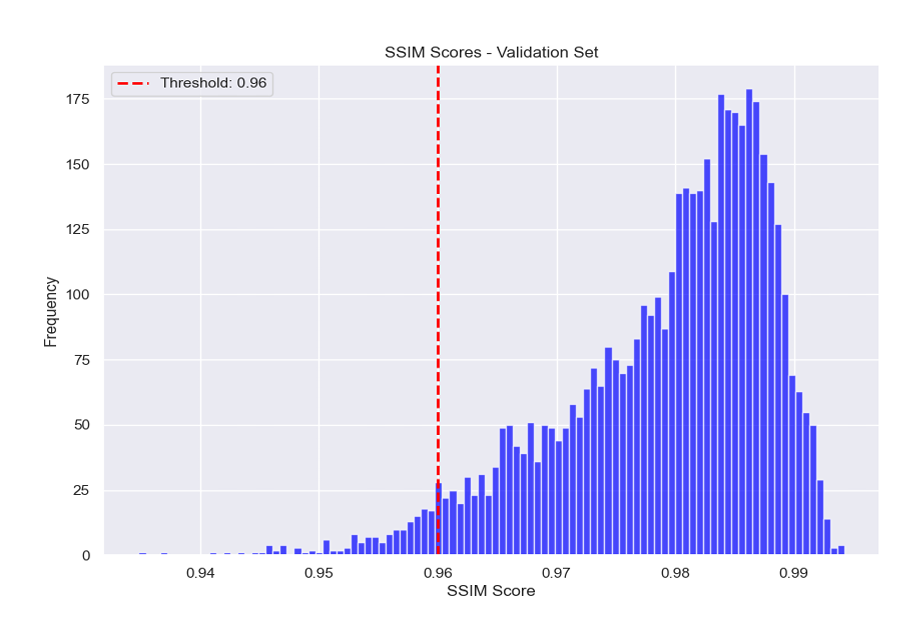
\includegraphics[width=\textwidth]{images/fig15.png}
\caption{SSIM threshold selection for IEEE Dataport dataset (threshold chosen above 0.96).}
\label{fig:fig15}
\end{figure}

\editornote{(65a) Reformatted caption to use sentence case and adhere to IEEE style;
(65b) Reordered phrasing for clarity: moved dataset name before threshold detail;
(65c) Removed redundant comma after “dataset” and replaced informal phrasing (“threshold here chosen”) with “threshold chosen above 0.96” for smoother academic tone;
(65d) Added final period to complete the caption grammatically, per IEEE guidelines.}

\begin{figure}[H]
\centering
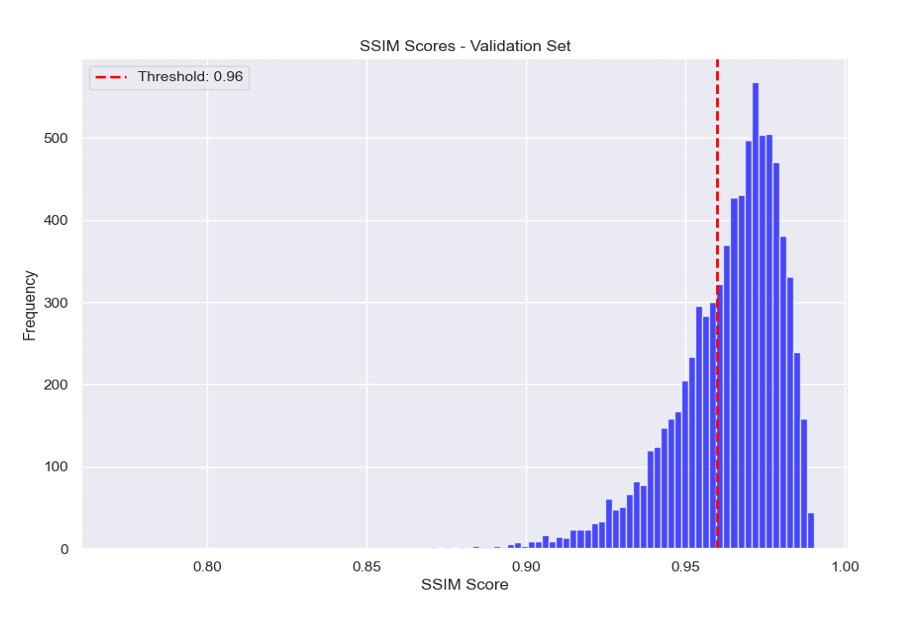
\includegraphics[width=\textwidth]{images/fig16.png}
\caption{SSIM threshold selection for Bounding Box Kaggle dataset, with threshold chosen above 0.96.}
\label{fig:fig16}
\end{figure}
  
\editornote{(66a) Reformatted caption to sentence case to align with IEEE style;
(66b) Reordered phrasing to lead with the method description (“SSIM threshold selection”) and moved the dataset name for clarity;
(66c) Reworded “threshold here chosen above 0.96” as “with threshold chosen above 0.96” for smoother tone and technical readability;
(66d) Added final period to complete the caption as per IEEE caption punctuation standards.}

\begin{table}[H]
  \caption{Evaluation metrics across various models and datasets.}
  \label{table:eval_metrics}
  \centering
  \begin{tabular}{l|c|c|c|c|c}
    \hline
    \textbf{Metric} &
    \makecell[c]{OC Autoencoder\\(IEEE Dataport)} &
    \textbf{Autoencoder} &
    \textbf{CNN} &
    \makecell[c]{Transfer\\Learning} &
    \makecell[c]{OC Autoencoder\\(Bounding Boxes)} \\
    \hline
    Accuracy & 0.99 & 0.9531 & 0.9728 & 0.948 & 0.99 \\
    Recall (Sensitivity) & 0.99 & 0.9528 & 0.9515 & -- & 0.97 \\
    Specificity & 0.99 & -- & 0.9962 & -- & 0.99 \\
    Precision & 0.99 & 0.9626 & 0.9960 & -- & 0.99 \\
    F1-score & 0.99 & 0.9577 & 0.9732 & -- & 0.98 \\
    \hline
  \end{tabular}
\end{table}

\editornote{
(67a) Added descriptive \textbackslash caption in sentence case per IEEE style;
(67b) Used \textbackslash makecell to wrap long column headers and avoid page overflow;
(67c) Applied sentence case to leftmost "Metric" column for clarity;
(67d) Retained boldface for “TABLE I: EVALUATION METRICS” for visual emphasis;
(67e) Used en dashes (–) to denote unavailable values, maintaining clear distinction from zero;
(67f) Final layout now renders within column bounds and maintains visual balance.
}

\section{Conclusion}
Malaria is a life-threatening disease, and early diagnosis is critical for saving lives. The accuracy of malaria detection from blood smear images often depends on the skill of medical professionals and the quality of available diagnostic tools. This dependency can place a significant burden on healthcare providers in rural areas with limited medical infrastructure. Deep learning methods that offer high diagnostic accuracy can help alleviate this strain by improving the speed and reliability of the diagnostic process. The proposed one-class autoencoder method shows promise as an effective decision-support tool for medical practitioners, particularly in resource-limited settings.

\editornote{
(68a) Recast opening sentence to “Malaria is a life-threatening disease, and early diagnosis is critical for saving lives” for smoother cadence and precision;
(68b) Rephrased “relies on the efficiency of medical professionals and the quality of instruments” as “depends on the skill of medical professionals and the quality of available diagnostic tools” for clarity and formality;
(68c) Replaced “can put a heavy strain” with “can place a significant burden” for more professional tone;
(68d) Reworded “make the diagnostic process easier and faster” as “improving the speed and reliability...” to elevate register;
(68e) Recast final sentence as “shows promise as an effective decision-support tool” to avoid promotional tone while maintaining a positive conclusion.}

In addition, the proposed method—a one-class autoencoder—addresses a common limitation in many classification models: the scarcity of abnormal instances. Because the autoencoder is trained exclusively on normal images, it learns to identify abnormalities by detecting deviations from the learned distribution. This approach enables the model to achieve high accuracy even when trained on a relatively small dataset of normal instances.

\editornote{
(69a) Rephrased opening clause for clarity: “the proposed method; a one class autoencoder” became “the proposed method—a one-class autoencoder” with corrected punctuation and hyphenation;
(69b) Recast “helps solve the issue that most models face” as “addresses a common limitation in many classification models” to elevate formality;
(69c) Rephrased repetitive sentence structures (“images that are different from the normal images”) for conciseness and flow;
(69d) Combined and tightened final sentence to reduce redundancy and improve technical clarity;
(69e) Used “deviations from the learned distribution” for more precise ML terminology.}

\newpage
\bibliographystyle{IEEEtran}
\bibliography{references}
\editornote{(70a) I noticed entry [11] had "year" instead of an actual year - I kept the access date.}
\end{document}
